\documentclass[landscape]{article}
\usepackage[pdftex]{graphicx}
\pagestyle{empty}
\oddsidemargin  -0.5 in
\evensidemargin -0.5 in
\headheight     0 in
\topmargin      -1 in
\textheight     7.7 in
\textwidth      10 in
\begin{document}
\large
\renewcommand{\labelitemi}{-}
\setlength{\parindent}{0 cm}

\begin{center} 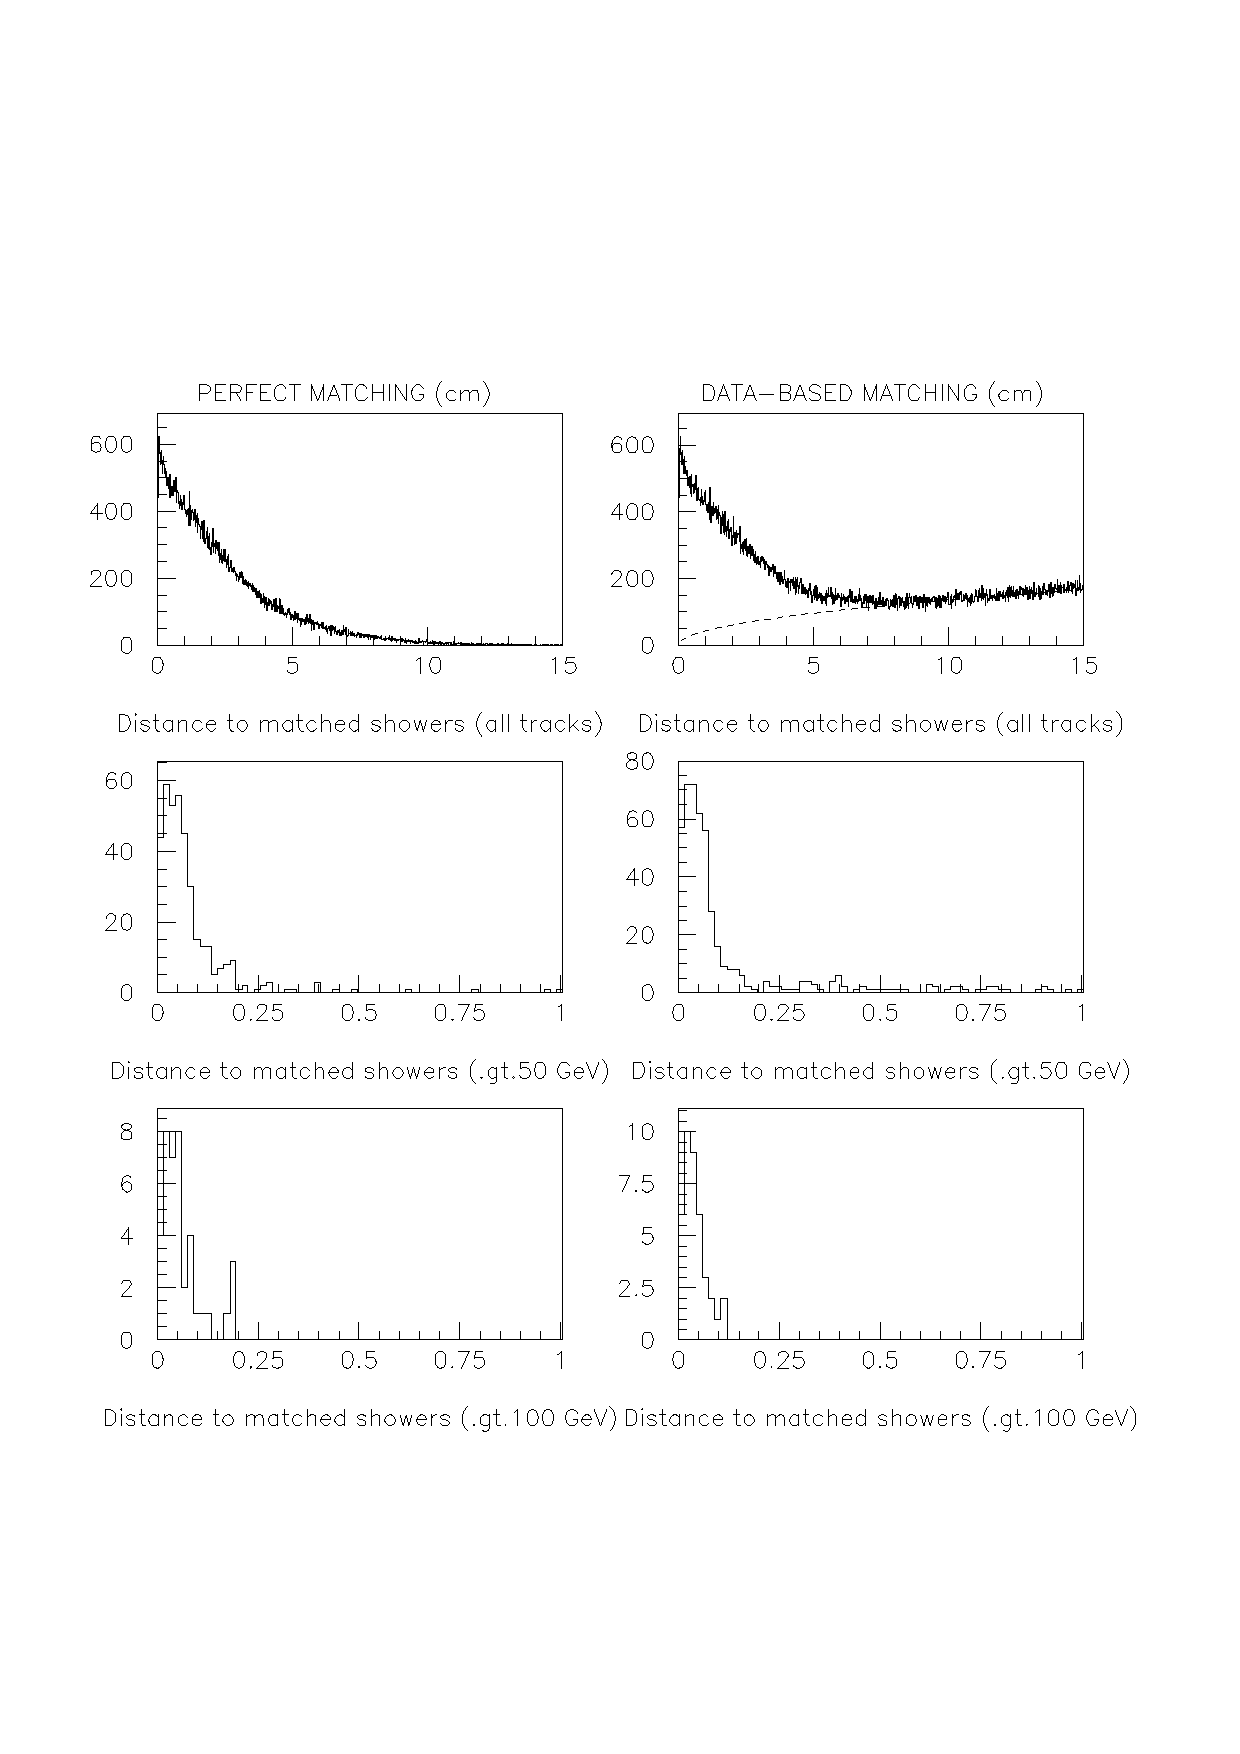
\includegraphics[height=0.8\textheight]{mcvsdata_matching.pdf} \end{center}

We have two new producers for track/cluster matching!

\vspace{0.2 cm}
{\tt LCDPerfectTrackClusterMatchingProd} and {\tt LCDTrackClusterMatchingProd}
have the same interface, but the former does MC truth matching and the
latter finds the closest track to a given cluster.

\vspace{0.2 cm}
Distance to closest shower distribution is wide for all tracks
(default cut is 5 cm), but it is much narrower (2 mm!) for very
energetic tracks.

\vspace{0.2 cm}
(Fakes under data-matched particles are above assumed to scale as $\sqrt{r}$.)

\pagebreak

\begin{center} \includegraphics[height=0.8\textheight]{withmatching_1.pdf} \end{center}

{\Large \bf Progressing through $\mbox{$\chi^0$}_1 \mbox{$\chi^0$}_3$ cuts (red is signal):}

\vspace{0.2 cm}
Now that we have isolated showers determined from data, we can
redefine missing energy as $\Sigma$ isolated showers + $\Sigma$ all
tracks.  The result is nearly the same as Laura's MC truth-matching.

\vspace{0.2 cm}
Put a cut at 300 GeV.

\vspace{0.2 cm}
(The vertical axis is 500 fb$^{-1}$ / 100 bins.)

\pagebreak

\begin{center} 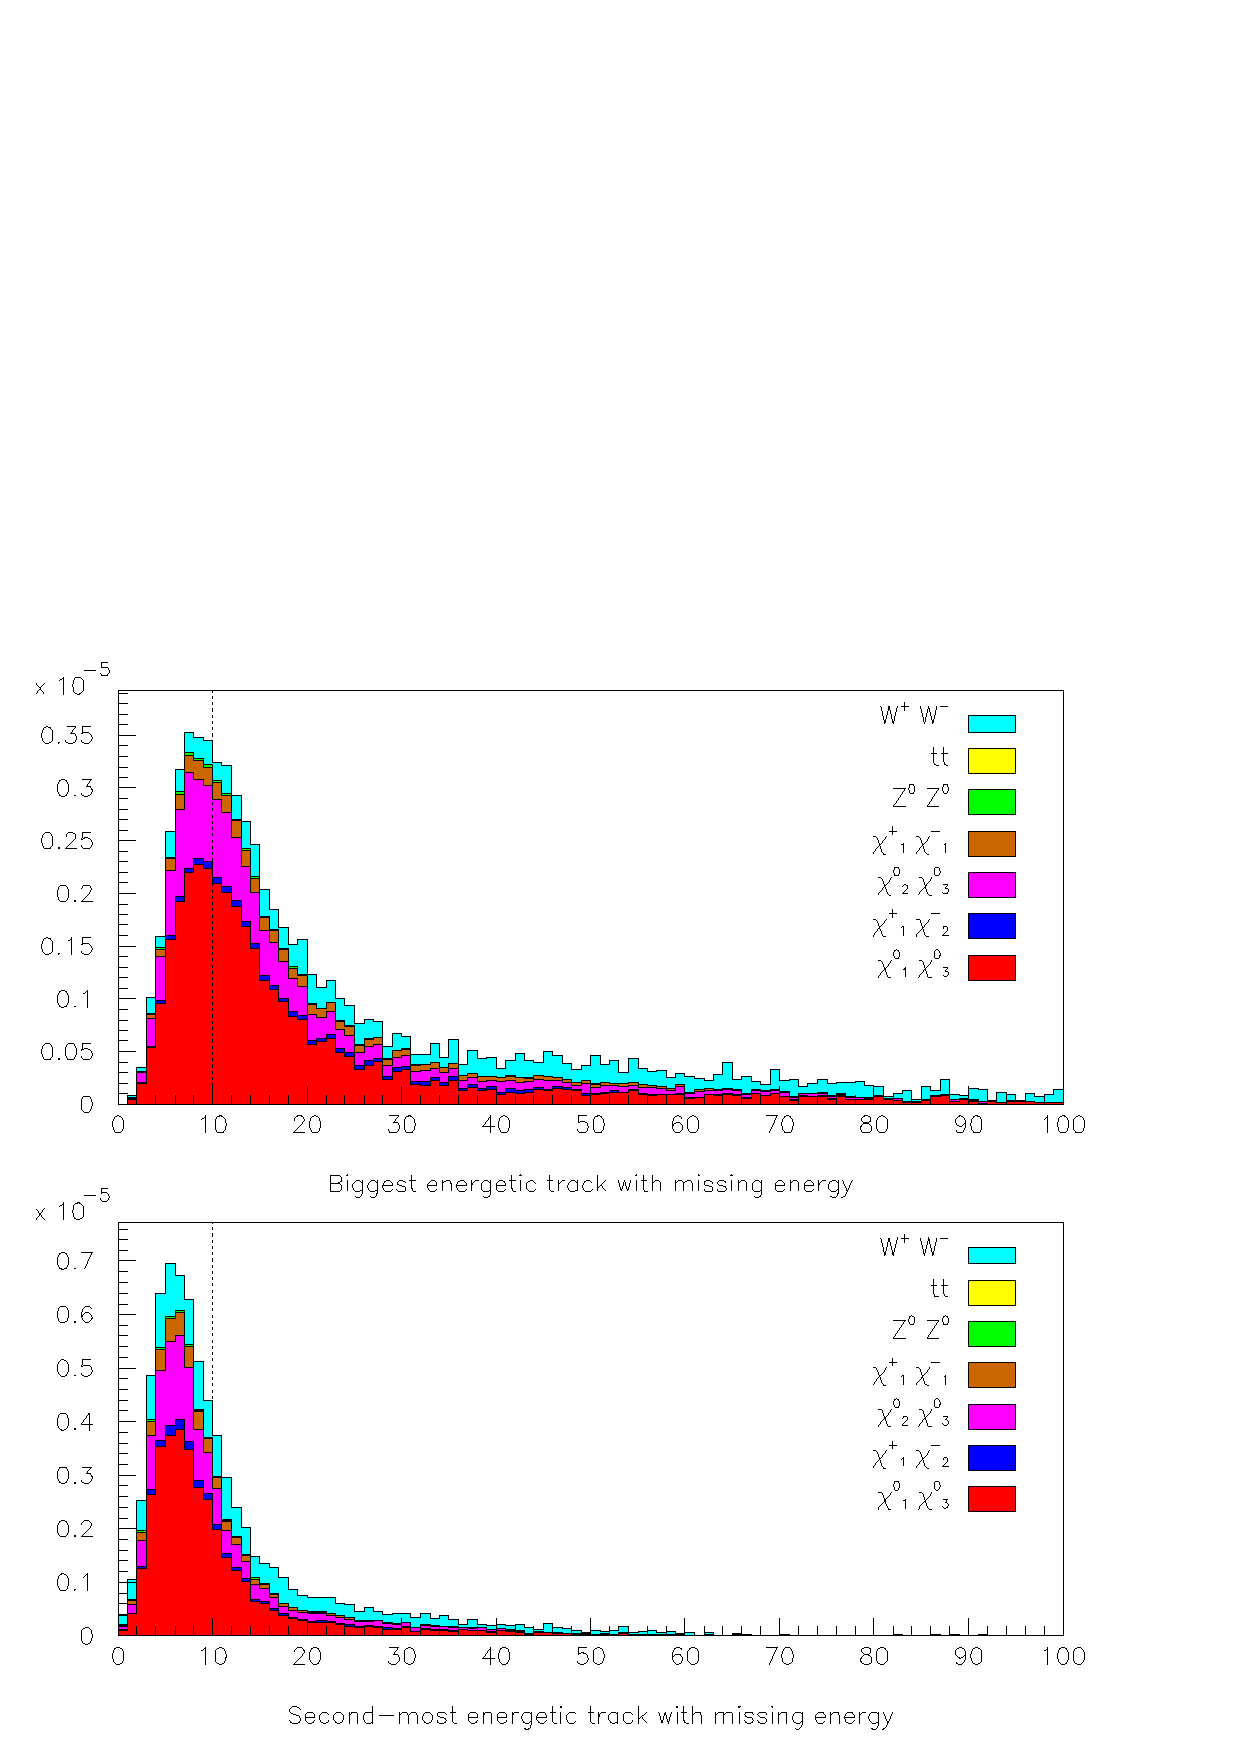
\includegraphics[height=0.8\textheight]{withmatching_2.pdf} \end{center}

Discriminate against $\mbox{$\chi^0$}_2 \mbox{$\chi^0$}_3$ by
requiring top two tracks to have $>$ 10 GeV each.

\vspace{0.2 cm}
This also improves cluster matching signal to noise (re: first slide).

\vspace{0.2 cm}
(These are {\it post-}discovery cuts.)

\pagebreak

\begin{center} \includegraphics[height=0.8\textheight]{withmatching_3.pdf} \end{center}

Back to missing energy as a touchstone: $\mbox{$\chi^0$}_2
\mbox{$\chi^0$}_3$ contamination above 300 GeV reduced.

\pagebreak

\begin{center} 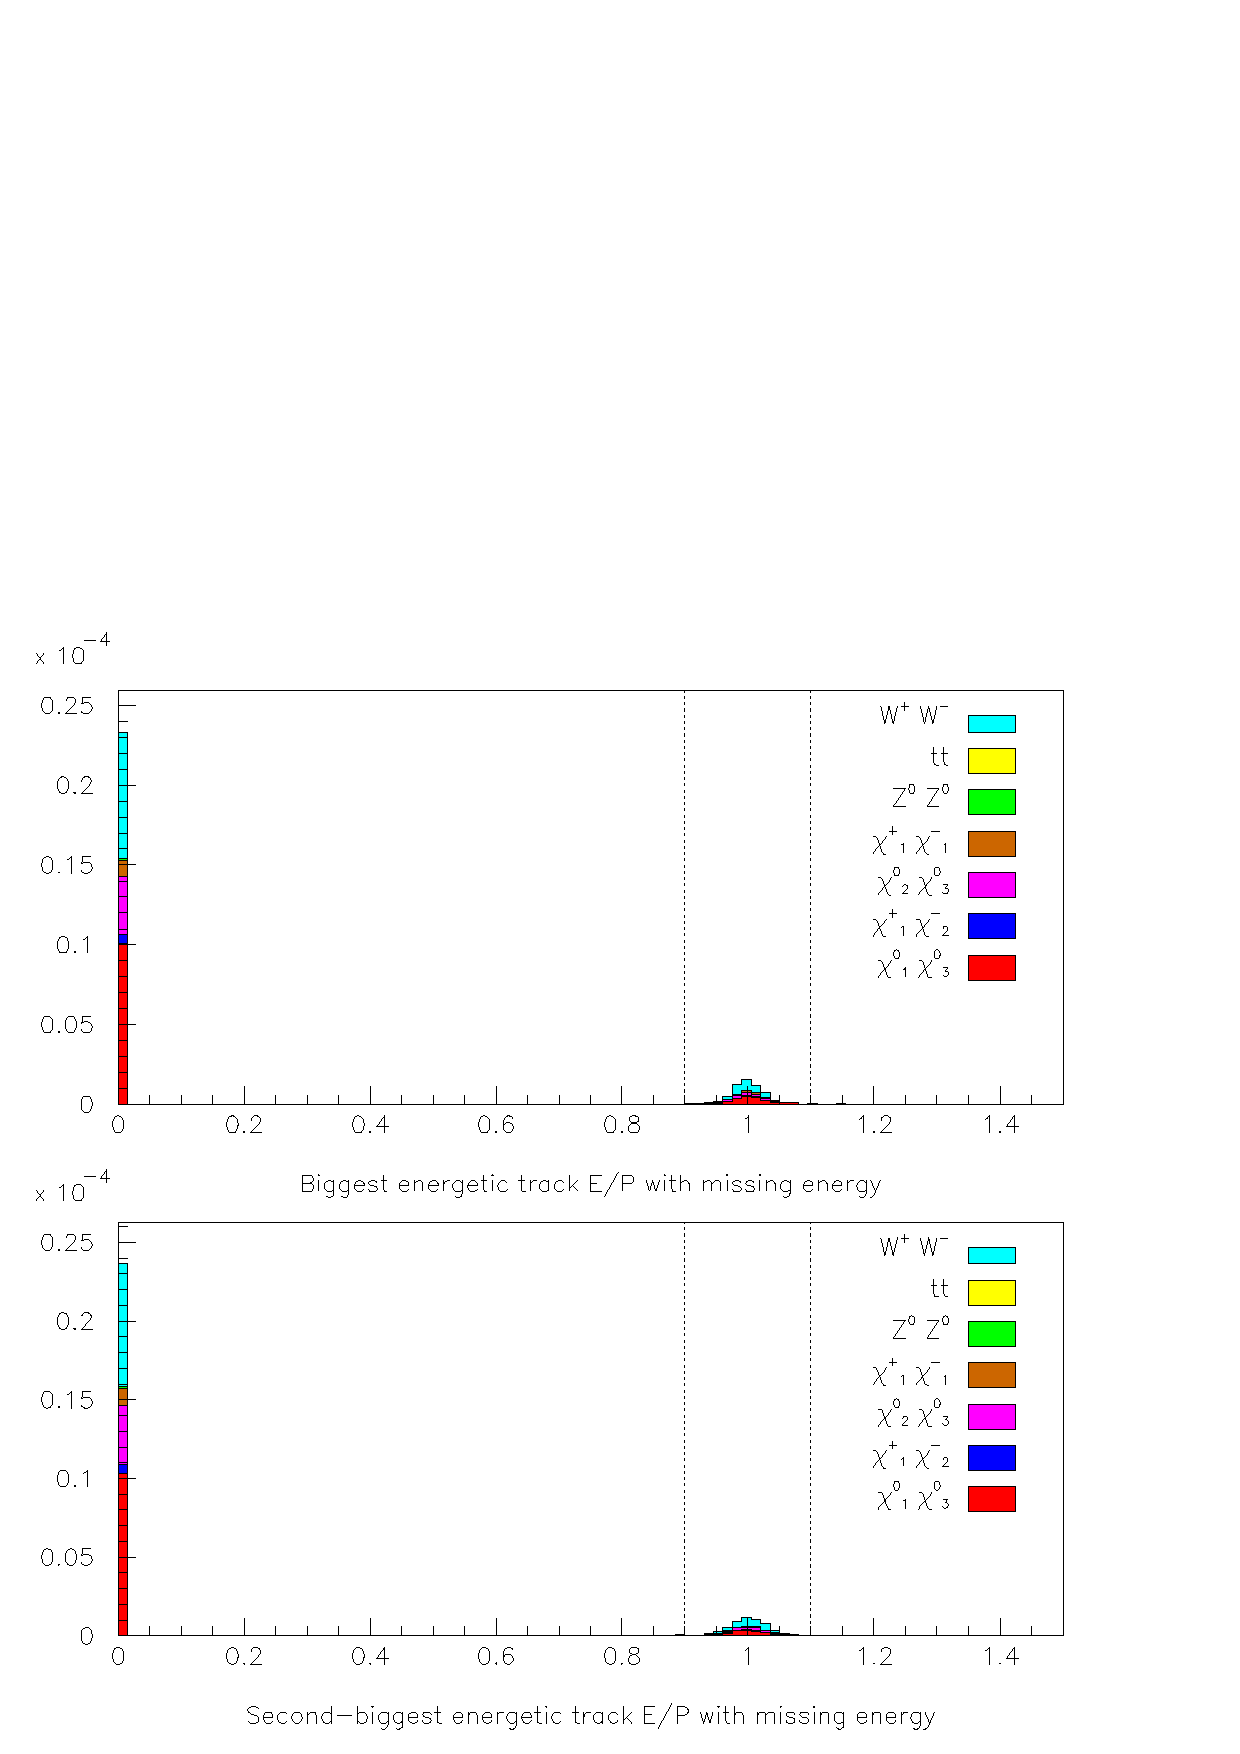
\includegraphics[height=0.8\textheight]{withmatching_4.pdf} \end{center}

Divide $Z^0Z^0$ background in four and signal in half by requiring
that both high-energy particles be electrons.

\vspace{0.2 cm}
As Laura noticed earlier, each MC particle produces a shower in the EM
calorimeter {\it xor} the hadron calorimeter, making it easy to
identify electrons but very hard to identify muons.  Presumably, there
will be some efficient way to identify muons at the linear collider:
so presumably we could double this, losing no signal.

\pagebreak

\begin{center} \includegraphics[height=0.8\textheight]{withmatching_5.pdf} \end{center}

Now look at the missing energy distribution.  It's maybe more than
half signal!

\pagebreak

\begin{center} 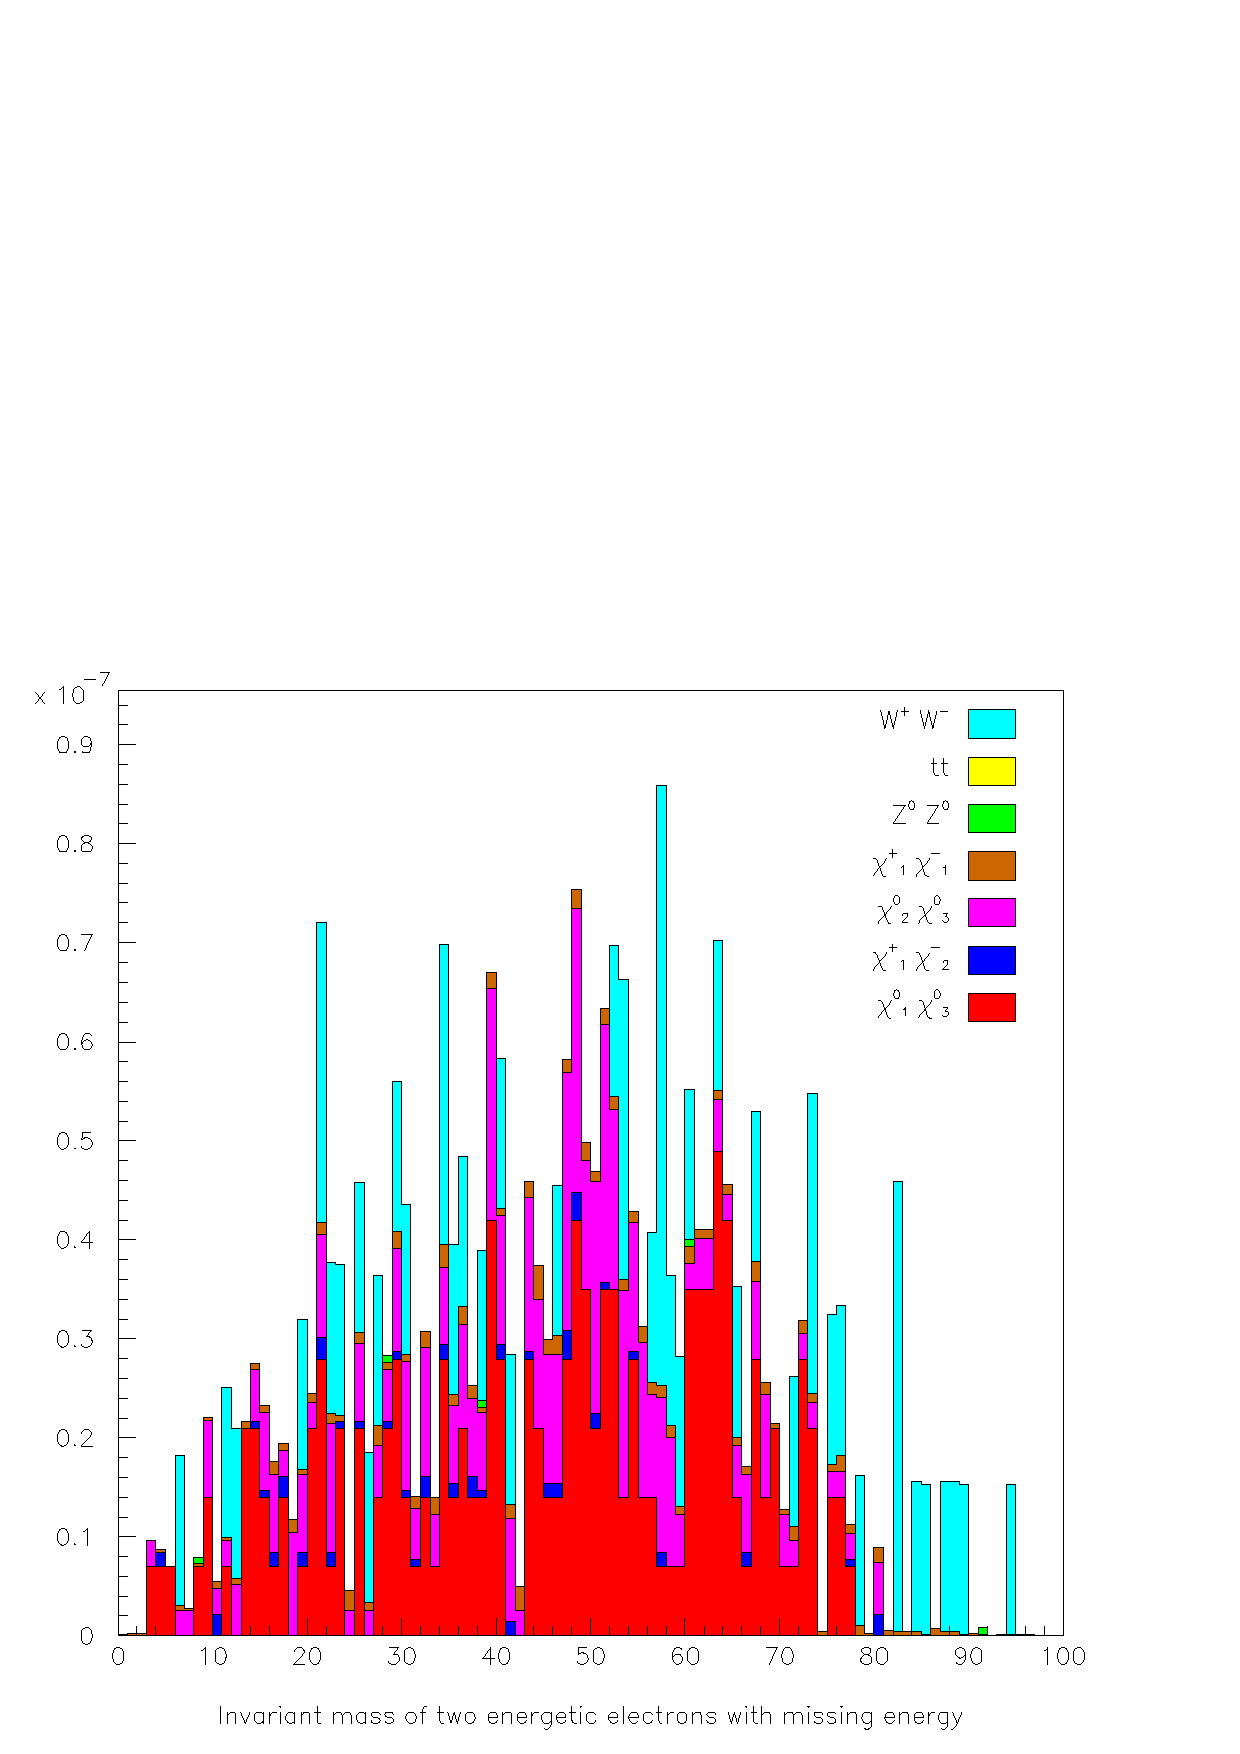
\includegraphics[height=0.8\textheight]{withmatching_6.pdf} \end{center}

This is the invariant mass distribution of the top two electrons.
We're looking for the cut-off at 80 GeV.

\pagebreak

\begin{center} 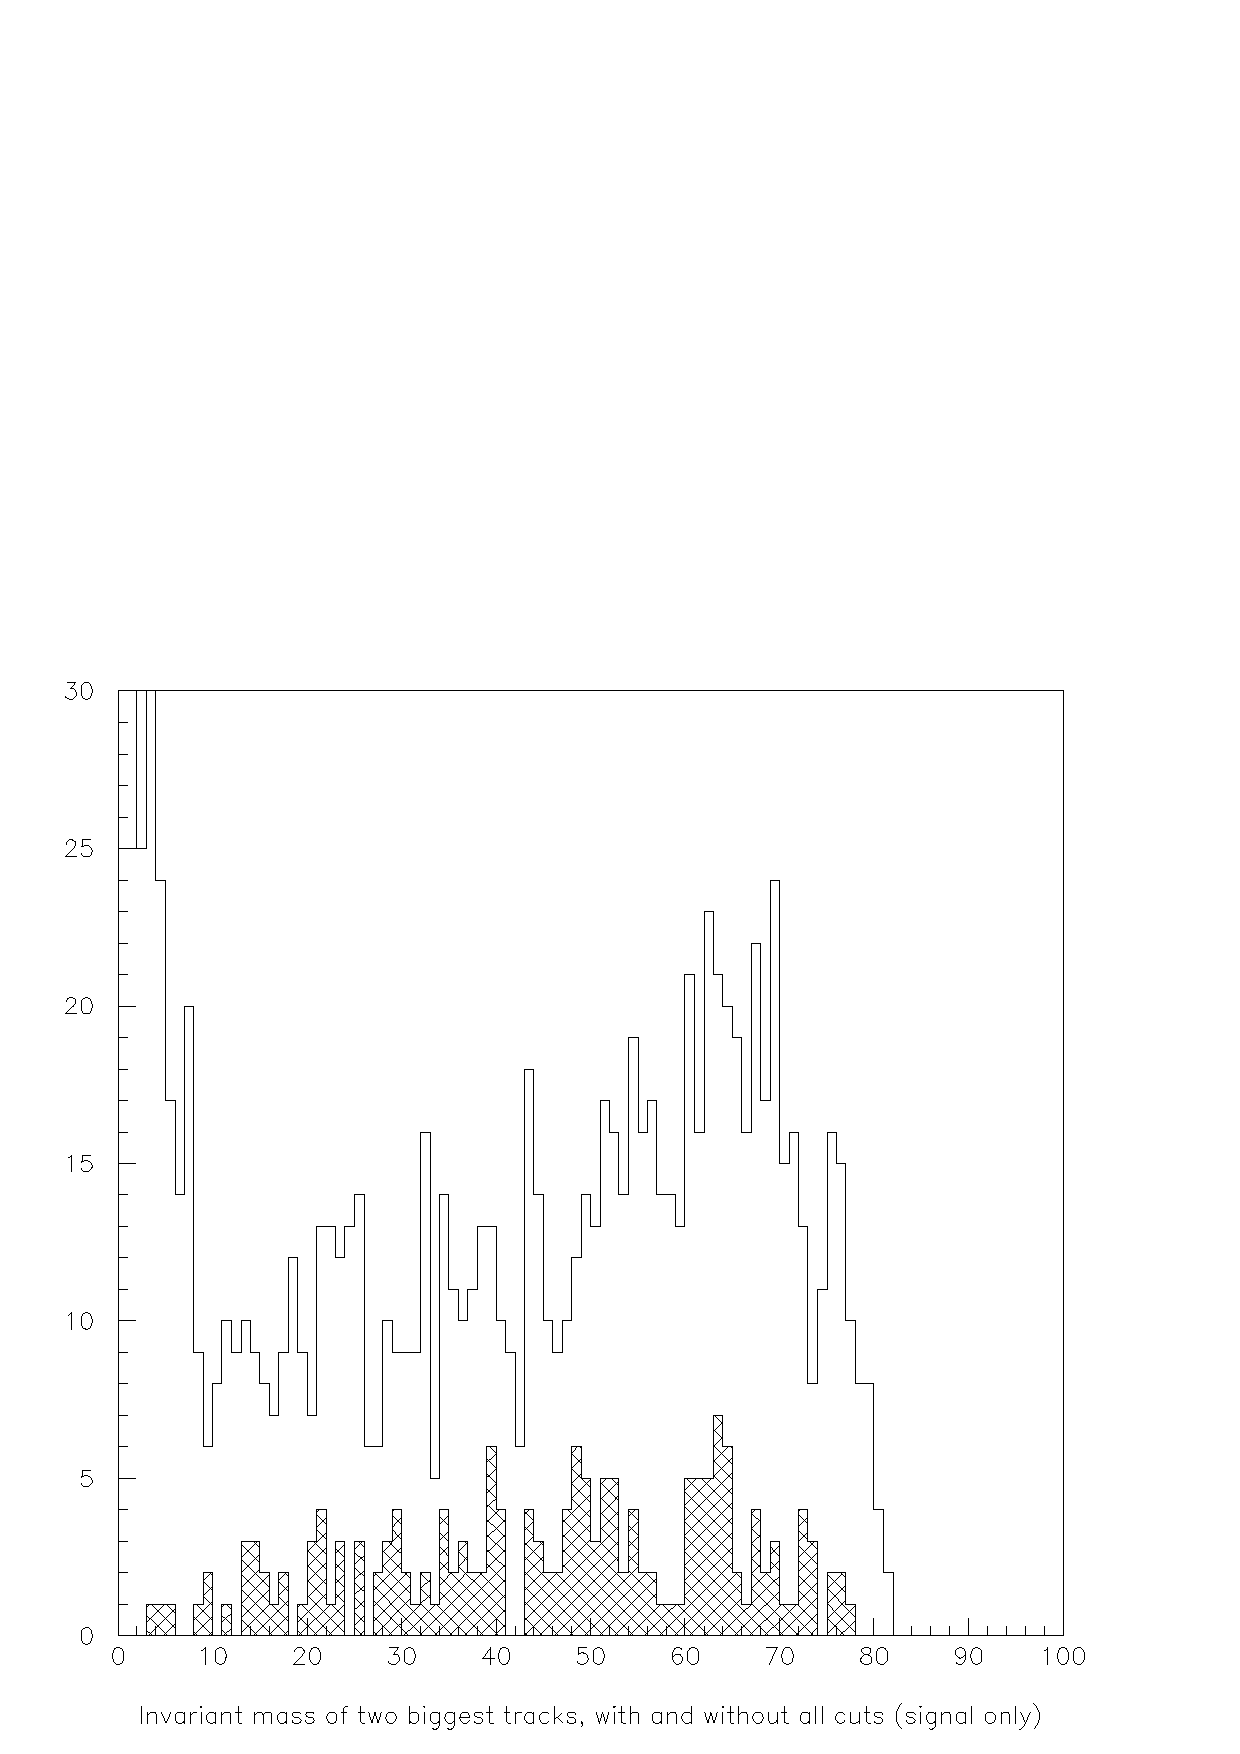
\includegraphics[height=0.8\textheight]{withmatching_7.pdf} \end{center}

The cut-off isn't significantly shifted by our cuts.  (The gap is
statistical fluctuations in the small signal MC sample.)

\end{document}
